% ---------------------------------------------------------------------------
% Author guideline and sample document for EG publication using LaTeX2e input
% D.Fellner, v1.13, April 29, 2009

\documentclass{egpubl}
\usepackage{sigrad13}

% --- for  Annual CONFERENCE
% \ConferenceSubmission % uncomment for Conference submission
% \ConferencePaper      % uncomment for (final) Conference Paper
% \STAR                 % uncomment for STAR contribution
% \Tutorial             % uncomment for Tutorial contribution
% \ShortPresentation    % uncomment for (final) Short Conference Presentation
%
% --- for  CGF Journal
% \JournalSubmission    % uncomment for submission to Computer Graphics Forum
% \JournalPaper         % uncomment for final version of Journal Paper
%
% --- for  EG Workshop Proceedings
\WsSubmission    % uncomment for submission to EG Workshop
% \WsPaper         % uncomment for final version of EG Workshop contribution
%
 \electronicVersion % can be used both for the printed and electronic version

% !! *please* don't change anything above
% !! unless you REALLY know what you are doing
% ------------------------------------------------------------------------

% for including postscript figures
% mind: package option 'draft' will replace PS figure by a filname within a frame
\ifpdf \usepackage[pdftex]{graphicx} \pdfcompresslevel=9
\else \usepackage[dvips]{graphicx} \fi

\PrintedOrElectronic

% prepare for electronic version of your document
\usepackage{t1enc,dfadobe}

\usepackage{egweblnk}
\usepackage{cite}

% For backwards compatibility to old LaTeX type font selection.
% Uncomment if your document adheres to LaTeX2e recommendations.
% \let\rm=\rmfamily    \let\sf=\sffamily    \let\tt=\ttfamily
% \let\it=\itshape     \let\sl=\slshape     \let\sc=\scshape
% \let\bf=\bfseries

% end of prologue


%=====================================================================================

\usepackage{amsmath,bm}
\usepackage{amssymb}
\usepackage{amsfonts}
\usepackage{caption}
\usepackage{subcaption} 
\usepackage{enumerate}
%\usepackage{enumitem}
%\usepackage{color}
\usepackage[usenames,dvipsnames,svgnames]{xcolor}
\usepackage{balance}
\usepackage{marginnote}
\usepackage{algorithmic}
\usepackage{algorithm}

\DeclareMathAlphabet{\mathcal}{OMS}{cmsy}{m}{n}

\def\etal{\textit{et al.}}
\renewcommand\floatpagefraction{1.0}
\renewcommand\topfraction{1.0}
\renewcommand\bottomfraction{.9}
\renewcommand\textfraction{.1}
\setcounter{totalnumber}{20}
\setcounter{topnumber}{10}
\setcounter{bottomnumber}{10}
\definecolor{MyGreen}{rgb}{0,0.7,0}
\definecolor{MyWhite}{rgb}{1,1,1}
\definecolor{MyGray}{rgb}{0.5,0.5,0.5}
\definecolor{LightGray}{rgb}{0.7,0.7,0.7}
\definecolor{DarkGray}{rgb}{0.3,0.3,0.3}
\definecolor{DarkYellow}{rgb}{0.7,0.7,0.0}
\definecolor{MyNavyBlue}{rgb}{0.2,0.3,0.7}
\newcommand{\black}[1]{{\color{Black} #1}}
\newcommand{\white}[1]{{\color{MyWhite} #1}}
\newcommand{\gray}[1]{{\color{MyGray} #1}}
\newcommand{\red}[1]{{\color{red} #1}}
\newcommand{\green}[1]{{\color{MyGreen} #1}}
\newcommand{\blue}[1]{{\color{MyNavyBlue} #1}}
\newcommand{\yellow}[1]{{\color{DarkYellow} #1}}
\newcommand{\maybe}[1]{\yellow{#1}}
\newcommand{\rout}[1]{\red{\sout{#1}}}
\newcommand{\repl}[2]{\rout{#1} \green{#2}}
\newcommand{\fix}[1]{\red{\emph{(#1)}}}
\newcommand{\Fix}[1]{\begin{itemize} \renewcommand\labelitemi{\red{--}} \item \red{#1} \end{itemize}}


% ---------------------------------------------------------------------
% EG author guidelines plus sample file for EG publication using LaTeX2e input
% D.Fellner, v1.17, Sep 23, 2010


\title[PMS]%
      {Poor Man's Rendering Of Segmented Data}

% for anonymous conference submission please enter your SUBMISSION ID
% instead of the author's name (and leave the affiliation blank) !!
\author[S. Lindholm \& A. Bock]
       {Stefan Lindholm$^{1}$
        and Alexander Bock$^{1}$
        \\
% For Computer Graphics Forum: Please use the abbreviation of your first name.
         $^1$Scientific Visualization Group, Link\"{o}ping University, Sweden
       }

% ------------------------------------------------------------------------

% if the Editors-in-Chief have given you the data, you may uncomment
% the following five lines and insert it here
%
% \volume{27}   % the volume in which the issue will be published;
% \issue{1}     % the issue number of the publication
% \pStartPage{1}      % set starting page


%-------------------------------------------------------------------------
\begin{document}

% \teaser{
%  \includegraphics[width=\linewidth]{eg_new}
%  \centering
%   \caption{New EG Logo}
% \label{fig:teaser}
% }

\maketitle

\begin{abstract}
In this paper we present a set of techniques for fast and efficient rendering of segmented data. Our approach utilizes the expected difference between two co-located samples of a label volume, taken with different interpolation kernels, to estimate a feature boundary. This allows us to achieve smooth class boundaries without, as with previous methods, needing to sample all eight neighbors in the label volume. 

\begin{classification} % according to http://www.acm.org/class/1998/
\CCScat{Computer Graphics}{I.3.3}{Picture/Image Generation}{Line and curve generation}
\end{classification}

\end{abstract}




\def\myitem{\diamond}




%-------------------------------------------------------------------------
\section{Introduction}

Rendering of segmented data is a core topic in the field of volume rendering. It is characterized in that it utilized external sources for the classification of grid points, rather than relying on user driven classification through, for example, a transfer function. By spending more resources on the classification as a pre-process step, much more reliable feature boundaries can be identified than what is possible through classification schemes applied at rendering time. Naturally, the topic of rendering segmented data is closely related to that of the actual segmentation. In this paper however, we assume that a full segmentation has been performed such that the \emph{source data} is complemented with a \emph{label volume}, i.e. an integer volume of the same dimensionality of the source data with a single per-voxel label denoting the class membership (material) of the voxel.

The basic idea behind rendering segmented data is identical to standard volume rendering: to select visual parameters based on the class membership of each sample. This is greatly simplified since the required class membership can be accessed directly though the label volume. Therefore, the visual properties are often defined on a per-class basis, rather than in a single global definition for the entire data. The complexity of the per-class visual properties vary depending on what the situation requires and can span from a unique color to a fully defined class-specific transfer function. In this paper we use a single transfer function per class but apply the same shading scheme to all classes, however, it should be noted that this is a stylistic choice rather than a requirement of the approach.

A problem that arises when rendering segmented data is that the basic approach to `just sample the label volume' to extract class memberships is not as straight forward as one might think. The simplest solution is, of course, to apply nearest neighbor sampling, which is guaranteed to return a valid class membership. Unfortunately, this leads to boundaries with a very blocky appearance (see Figure~\ref{fig:nearestexample}). The membership operation is said to have \emph{voxel-resolution}. The most intuitive way to achieve a higher, \emph{pixel-resolution}, membership operation is naturally to allow for interpolation when sampling the label volume. This is, however, not guaranteed to return a valid class label unless there is no more than two classes in the entire volume. For example, an interpolation in a boundary area between class $3$ and class $5$ would return a class label of $4$ even if this was not existent at that particular location in the data (see Figure~\ref{fig:linearexample}). An approach to achieve a pixel-resolution membership operation for segmented data, called two-level volume rendering, was presented in \cite{Hadwiger2003}. In this approach, all eight neighboring grip points in the label volume are sampled to acquire the information necessary to remap the $3$--$5$ operation to a $0$--$1$ range and thereby avoid illegal interpolations. The result is much smoother boundary representations that are more visually pleasing. Unfortunately, the method requires an additional \emph{seven} samples per step along the ray which is many times unfeasible.

In this paper we present a novel method that delivers results comparable to pixel-resolution schemes while only requiring a \emph{single} extra sample. The core of our approach is to sample the level volume twice at the same location, with and without interpolation. The difference between the two values is then used to smoothen the visual representation near class boundaries without creating incorrectly interpolated class values. We show that our method produces results visually comparable to methods that utilize full neighborhood sampling while requiring a factor of $7:1$ less additional samples. Additionally, we also present a data compression approach that removes the need to have the label volume accessible during rendering.

%-------------------------------------------------------------------------
\section{Poor Man's Rendering With Label Volume}

The implementation will be presented in three steps. First we provide details on how to sample a single texture with different interpolation kernels in OpenGL. We then present how to compute the actual class membership of each sample as well as the attenuation parameter $t$ that is used to smoothen the boundaries. 

\subsection*{Nearest Neighbor and Linear Sampling}

As previously noted, the implementation relies on sampling the the same volume twice with different interpolation kernels. For many architectures, however, a single texture can only be associated with a single sampling mode. One way to get around this restriction is to always force the label volume to be associated with linear interpolation. The nearest neighbor sample can then be accessed by adding an offset that forces this sample directly to the center of the nearest voxel. The nearest grid point can be accessed as follows
\begin{align}
s_\mathrm{near} &= \mathrm{floor}\big(s + vec3(0.5)\big) \label{eq:near}  
\end{align}
where $s$ is the original sample position along the ray and $s_\mathrm{lin}$ is the position of the nearest neighbor. For OpenGL both samples can then be accessed through \texttt{texture3D}. Note, that OpenGL uses voxel centric values, as opposed to grid centric values, for \texttt{texture3D} and that the sample positions needs to be mapped accordingly.
\begin{align}
o &= \frac{0.5}{\mathrm{DataRes}}\\
s_\mathrm{vc} &= o + (1 - 2o) s_\mathrm{vc}
\end{align}
 Alternatively. the nearest neighbor sampling can be achieved through \texttt{texelFetch} which should not require any additional mapping of the sampling point.

Once the linear and nearest sample points have been computed, they are used to extract the linear and nearest values from the label volume, $l_\mathrm{lin}$ and $l_\mathrm{near}$ respectively.

\subsection*{Class Membership and Class Attenuation}

In our approach the class membership is directly decided by the nearest neighbor sample in the label volume, $l_\mathrm{lin}$. This means that membership itself is defined at voxel-resolution. To achieve smoother class boundaries we introduce a \emph{class attenuation parameter}, $t$.

The attenuation parameter is computed from the nearest and linear label values
\begin{align}
t &= \mathrm{abs}(l_\mathrm{lin} - l_\mathrm{near})  .  \label{eq:attenuation}
\end{align}
Looking at Equation~\ref{eq:attenuation}, we see that $t=0$ as long as the interpolated value is identical to the nearest neighbor value. This will be the case as long as the local neighborhood around the sample point only contains a single class. We can also note that if the local neighborhood contains two or more classes, then $t > 0$. The class attenuation parameter thereby functions as a boundary indicator.

Interpreting the attenuation parameter as a boundary indicator, we use it to adjust the opacity of the current sample. Ideally, we want full opacity when the samples are fully inside a single class and zero opacity when samples are half way in between two (or more) classes. Unfortunately, this requires us to know all classes that effect the interpolated value, which in turn would require us to sample the entire neighborhood in the label volume (which we don't want to do). Instead, we always map the opacity to zero as $t$ reaches $0.5$ 
\begin{align}
\alpha' &= (1-(2t)^2) \cdot \alpha  .  \label{eq:alpha}
\end{align}
The full process is described in Algorithm~\ref{code:1}.

\begin{algorithm}[t]
%\renewcommand{\thealgorithm}{1}
\caption{\label{code:1} \emph{Poor Man's Rendering \textbf{with} Label Volume}}
\begin{algorithmic}
\REQUIRE \quad\\
A source volume $V_\mathrm{src}$ and a label volume $V_L$,\\both present on the GPU\\
A set of labels $\{ l_1, l_2, \cdots, l_n \}$ \\
A transfer function, $\mathrm{TF}_i$ for each label $l_i$ 
\STATE \hspace{-3mm}\textbf{Algorithm:}
\FORALL {sample points along ray} \nonumber
\STATE $\myitem$ Sample $V_L$ using \emph{nearest neighbor} interp. $\rightarrow l_\mathrm{near}$
\STATE $\myitem$ Sample $V_L$ using \emph{linear} interpolation $\rightarrow l_\mathrm{lin}$
\STATE $\myitem$ Compute attenuation parameter $t$ according to Eq.~\ref{eq:attenuation}
\STATE $\myitem$ Compute alpha modulation according to Eq.~\ref{eq:alpha}
\STATE $\myitem$ Sample $V_\mathrm{src}$ using \emph{linear} interpolation $\rightarrow v_\mathrm{lin}$ 
\STATE $\myitem$ Select a TF based on $l_\mathrm{near}$
\STATE $\myitem$ Evaluate $\mathrm{TF}_\mathrm{near}(v_\mathrm{lin})$ 
\STATE $\myitem$ Apply alpha modulation to output
\STATE $\myitem$ Composite output to result
\ENDFOR
\end{algorithmic}
\end{algorithm}

While Equation~\ref{eq:alpha} largely achieves the desired effect, it is important to note that it introduces a few predictable irregularities (hence the title of the paper). First, $t=0.5$ only corresponds to the half way mark between two labels if their numerical labels are separated by a single unit (e.g. $1$--$2$, $3$--$2$). For all other cases, the opacity will reach zero before the half way mark. Second, in some rare corner cases, the nearest neighbor value may change before the opacity has reached zero, effectively creating a sharper than intended cutoff. In short, we have less fine-tuned control over the opacity behavior across boundary regions. 

What makes Poor Man's Rendering such an attractive trade-off is that the visual impact of the expected irregularities is near insignificant and thus acceptable given the increase in performance compared to the full neighborhood analysis.


\section{Poor Man's Rendering Without Label Volume}

In this section we present a data encoding scheme that eliminates the need to upload the label volume to the GPU. The encoding relies on a set of linear mappings (one for each class) from the source volume to an encoded target volume. The key here is to ensure that the co-domain of the mappings each span a unique value range in the target volume. 

For example, if we have three classes which voxels exhibit overlapping value ranges ($0.3$--$0.5$, $0.2$--$0.7$ and $0.1$--$0.5$). We then map the value ranges of of these classes to three unique value ranges in the target volume
\begin{align}
l_1&: [0.3,0.5] \mapsto [0.1,0.3] \nonumber\\
l_2&: [0.2,0.7] \mapsto [0.4,0.6] \nonumber\\
l_3&: [0.1,0.5] \mapsto [0.7,0.9] \nonumber  .
\end{align}
This makes it possible to determine the class of a sample solely based on which unique range it belong to. Note that interpolation in this volume can still lead to invalid results. The data encoding is performed as a pre-process step and the encoded volume replaces the source volume on the GPU. Meta information from the mappings also needs to be uploaded in order to decode the volume during rendering. The decoding process is simply the inverse of the linear mapping for each class. 

The computation of the attenuation parameter $t$ without a label volume works as follows. Two samples are taken from the encoded volume, with nearest neighbor ($e_\mathrm{near}$) and linear interpolation ($e_\mathrm{lin}$) respectively. First, the nearest neighbor sample is used to identify the label and its valid value range (from the uploaded mapping information)
\begin{align}
e_\mathrm{near} \rightarrow l_\mathrm{near},\; [e_\mathrm{min}, e_\mathrm{max}]  .
\end{align}
Based on this the attenuation parameter $t$ can be computed as 
\begin{align}
t &= \mathrm{abs}(v_\mathrm{lin} - \frac{e_\mathrm{max} + e_\mathrm{min}}{2}) - \frac{e_\mathrm{max} - e_\mathrm{min}}{2}  \label{eq:attenuation2}
\end{align}
clamped to the $0$--$1$ range. Poor Man's Rendering can now be performed using Equations~\ref{eq:attenuation2}~and~\ref{eq:alpha}. The full process is described in Algorithm~\ref{code:2}.

A positive side effect to the encoding is that the user can now specify a single global transfer function without labels while still maintaining separate visual properties for the different classes (since the value ranges are known to be non-overlapping). This is particularly beneficial for systems that are not preciously set up to load and render segmented data or multiple volumes. A potential issue with this type of encoding is the loss of precision that follows from the remapping. Since this naturally becomes a situational trade-off a complete analysis is out of the scope of this paper. What can be said is that as the more narrow the value ranges are per class in the source volume, the less precision will be lost. 


\begin{algorithm}[t]
%\renewcommand{\thealgorithm}{1}
\caption{\label{code:2} \emph{Poor Man's Rendering \textbf{without} Label Volume}}
\begin{algorithmic}
\REQUIRE \quad\\
A source volume $V_\mathrm{src}$ and a label volume $V_L$\\
A target volume for the encoding $V_\mathrm{enc}$\\
A set of labels $\{ l_1, l_2, \cdots, l_n \}$ \\
A transfer function, $\mathrm{TF}_i$ for each label $l_i$ 
\STATE \hspace{-3mm}\textbf{Pre-process:}
\FORALL {labels $l_i$} \nonumber
\STATE $\myitem$ Find the value range $[r_\mathrm{min}, r_\mathrm{max}]$ covered by by the voxels of class $i$ in $V_\mathrm{src}$
\STATE $\myitem$ Assign a unique range $[e_\mathrm{min},e_\mathrm{max}]$ where $e_\mathrm{min} = 0.1+0.3 i$ and $e_\mathrm{max} = 0.2+0.3 i$ in $V_\mathrm{enc}$
\STATE $\myitem$ Linearly map all voxels of class $i$ from $V_\mathrm{src} \mapsto V_\mathrm{enc}$ as $[r_\mathrm{min}, r_\mathrm{max}] \mapsto [e_\mathrm{min},e_\mathrm{max}]$
\STATE $\myitem$ Save mapping information as $M_i$
\ENDFOR
\STATE $\myitem$ Upload $V_t$ to GPU together with meta information of each class mapping
\STATE \hspace{-3mm}\textbf{Algorithm:}
\FORALL {sample points along ray} \nonumber
\STATE $\myitem$ Sample $V_\mathrm{enc}$ using \emph{nearest neighbor} interp. $\rightarrow e_\mathrm{near}$
\STATE $\myitem$ Identify current label $l_\mathrm{near}$ and valid value range $[e_\mathrm{min}, e_\mathrm{max}]$ based on which unique range that contains $e_\mathrm{near}$ 
\STATE $\myitem$ Sample $V_\mathrm{enc}$ using \emph{linear} interpolation $\rightarrow e_\mathrm{lin}$
\STATE $\myitem$ Compute attenuation parameter $t$ according to Eq.~\ref{eq:attenuation2}
\STATE $\myitem$ Compute alpha modulation according to Eq.~\ref{eq:alpha}
\STATE $\myitem$ Compute the inverse mapping $e_\mathrm{lin} \mapsto v_\mathrm{lin}$ using $M_j$
%\STATE $\myitem$ Select a TF based on $l_\mathrm{near}$ 
%\STATE $\myitem$ Evaluate $\mathrm{TF}_\mathrm{near}(v_\mathrm{lin})$
\STATE $\myitem$ Evaluate $\mathrm{TF}(v_\mathrm{lin})$ 
\STATE $\myitem$ Apply alpha modulation to output
\STATE $\myitem$ Composite output to result
\ENDFOR
\end{algorithmic}
\end{algorithm}


\begin{figure*}
\centering
\begin{minipage}{0.44\linewidth}
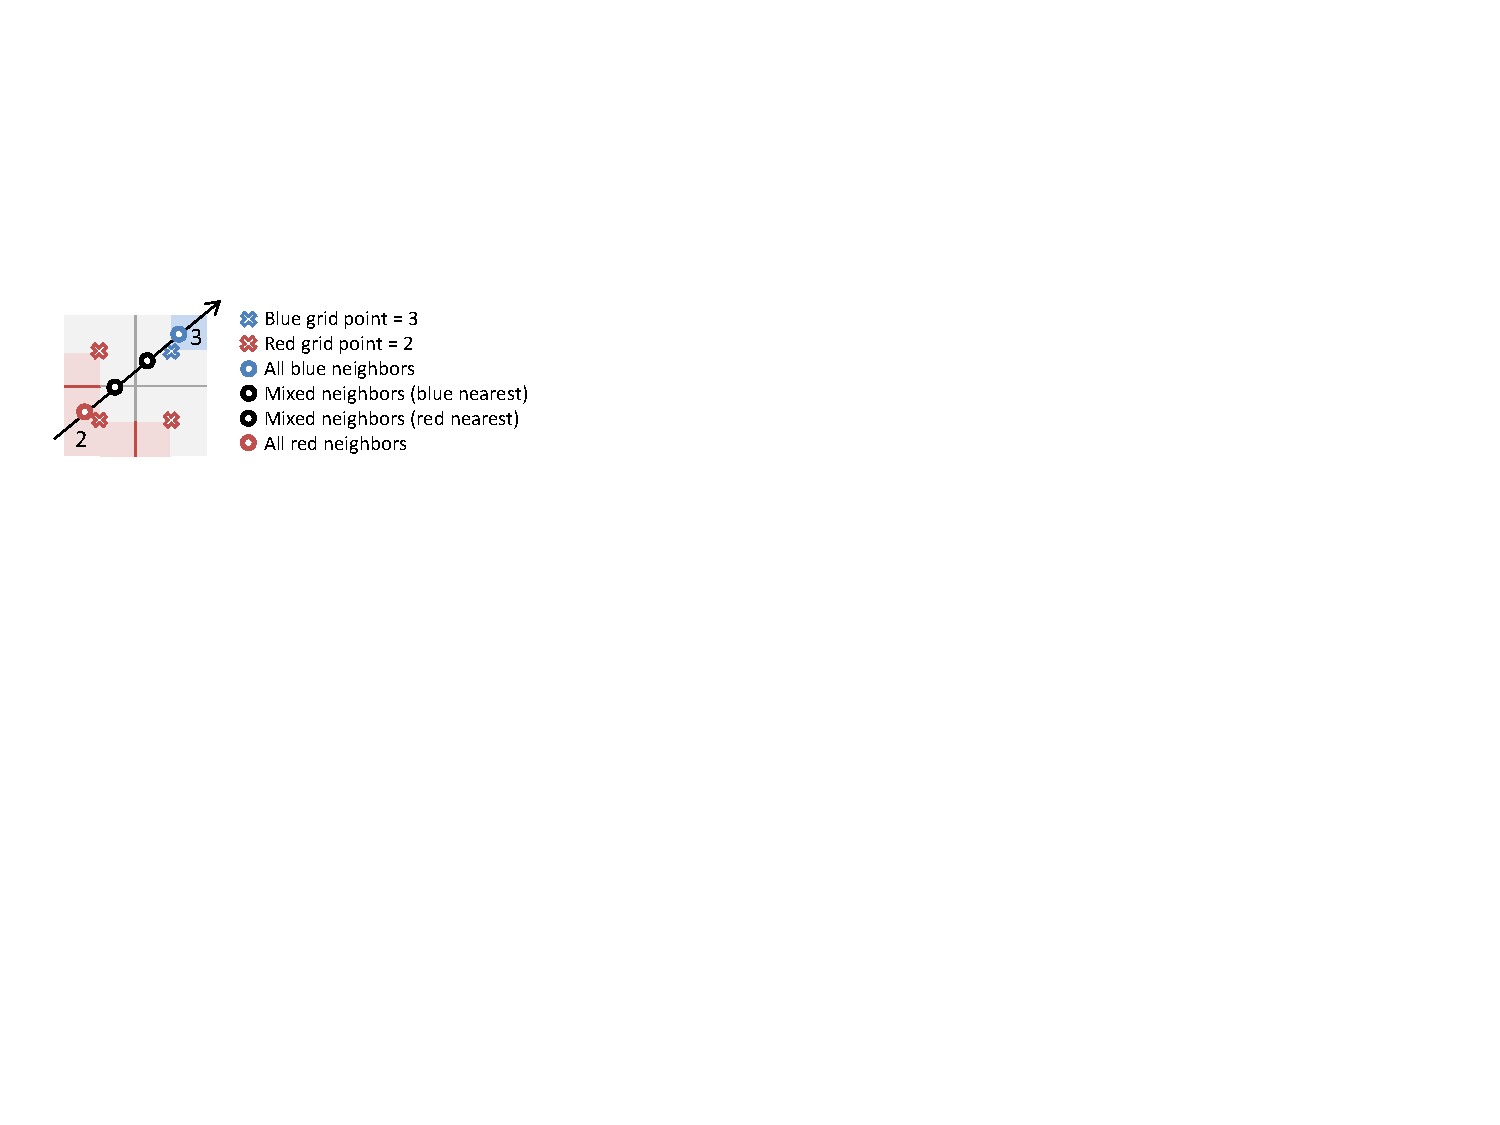
\includegraphics[width=1.0\linewidth]{figures/Neighborhood_all}
\end{minipage}\hfill
\begin{minipage}{0.27\linewidth}
\begin{minipage}{1.0\linewidth}
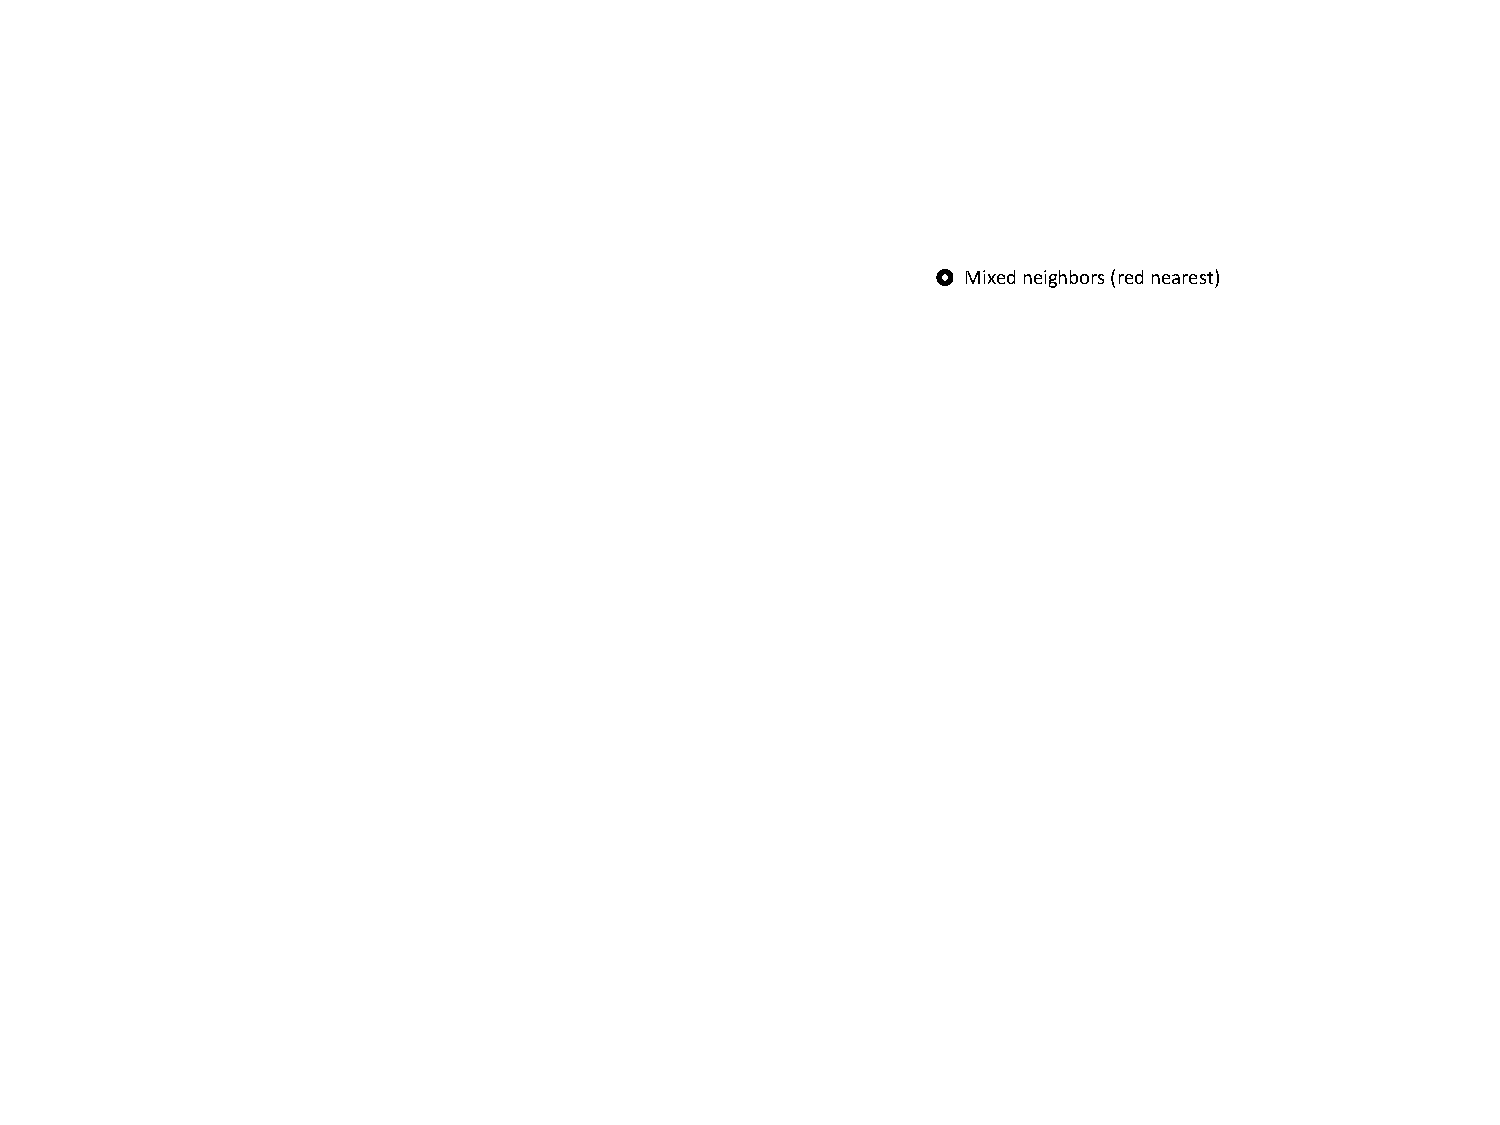
\includegraphics[width=1.0\linewidth]{figures/Neighborhood_red}
\end{minipage}
\begin{minipage}{1.0\linewidth}
\begin{align}
l_\mathrm{near} &= 2\nonumber\\
l_\mathrm{lin} &= 2.2\nonumber\\
t &= \frac{\mathrm{abs}(2.2-2)}{0.5}\nonumber\\
\alpha' &= \alpha \times (1-t^2) = 0.96 \times \alpha\nonumber
\end{align}
\end{minipage}
\end{minipage}\hfill
\begin{minipage}{0.27\linewidth}
\begin{minipage}{1.0\linewidth}
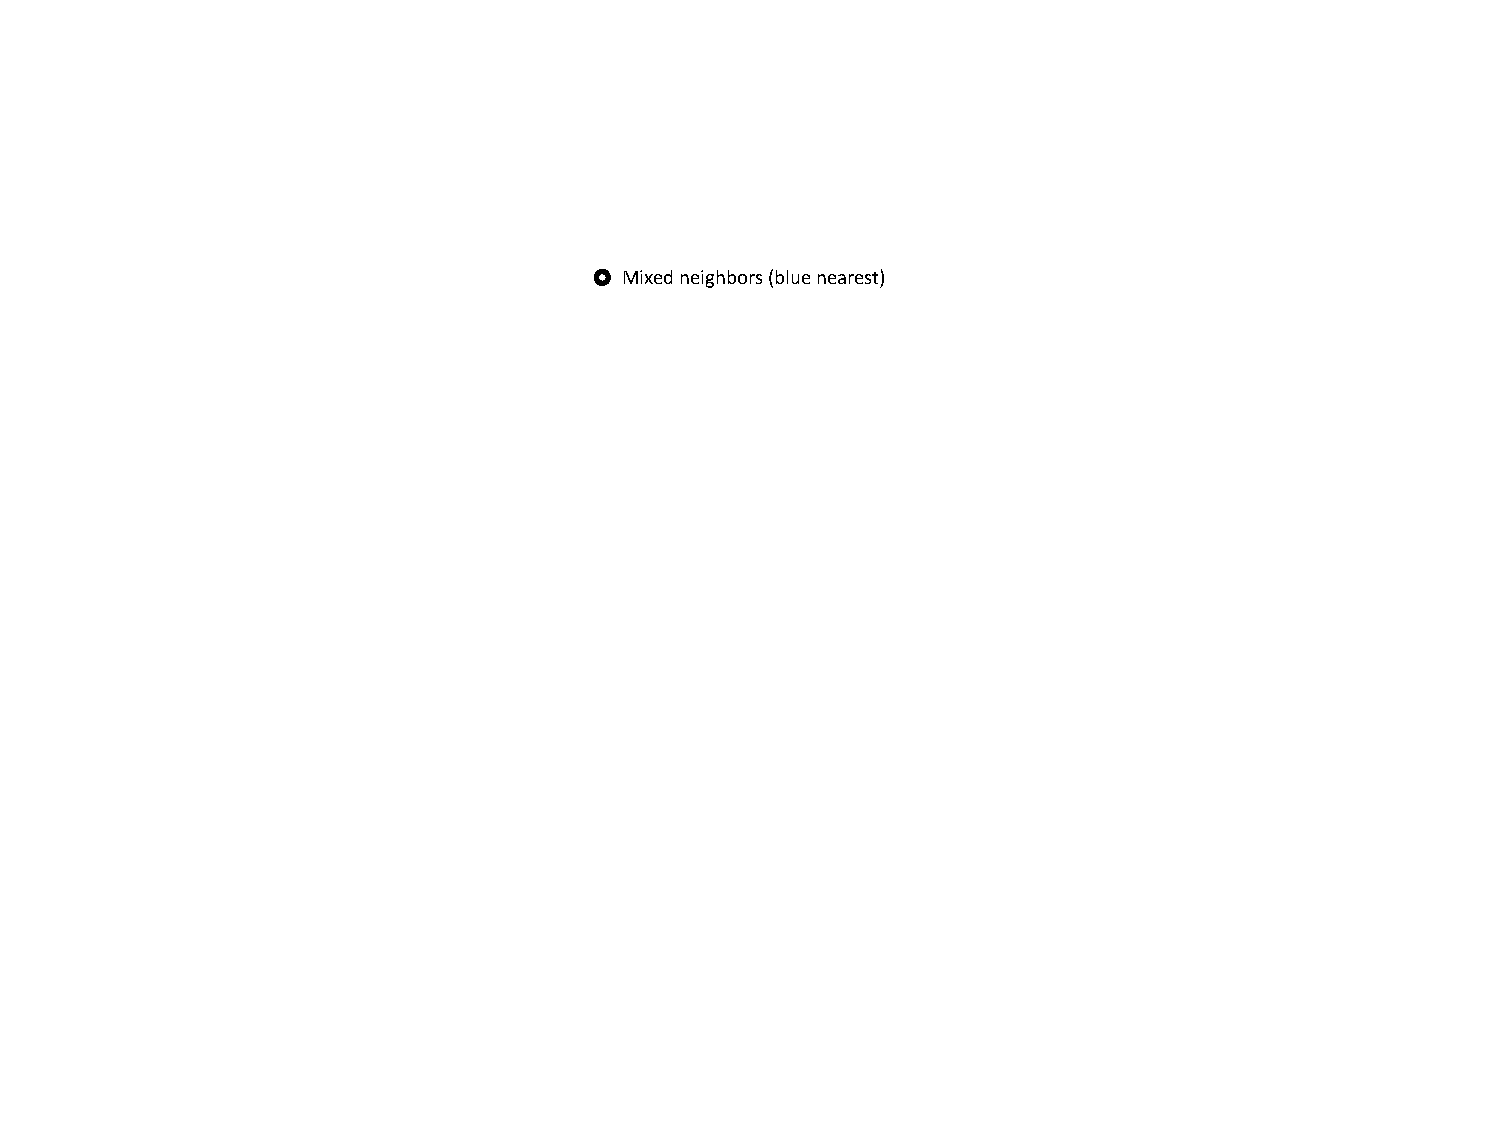
\includegraphics[width=1.0\linewidth]{figures/Neighborhood_blue}
\end{minipage}
\begin{minipage}{1.0\linewidth}
\begin{align}
l_\mathrm{near} &= 3\nonumber\\
l_\mathrm{lin} &= 2.6\nonumber\\
t &= \frac{\mathrm{abs}(2.6-3)}{0.5}\nonumber\\
\alpha' &= \alpha \times (1-t^2) = 0.36 \times \alpha\nonumber
\end{align}
\end{minipage}
\end{minipage}
\caption{\label{fig:example-illustration}
Example computations of ray contributions. The visible ray segment starts inside the red feature (class id 2), and ends inside the blue feature (class id 3). The class membership of the two samples taken in between the features needs to be decided. In our approach, their membership is fully determined by a nearest neighbor query in the label volume (here resulting in $l_\mathrm{near}=2$ and $l_\mathrm{near}=3$ respectively). However, in order to achieve smooth boundaries at pixel-resolution we employ an alpha modulation based on the difference between the the nearest query and another query using linear interpolation (here resulting in $l_\mathrm{near}=2.2$ and $l_\mathrm{near}=2.6$ respectively). 
}
\end{figure*}



%-------------------------------------------------------------------------
\subsection{Results}



%-------------------------------------------------------------------------
\subsection{Discussion}

In this paper we have presented an approach to achieve smooth boundary transitions when rendering segmented data while maintaining acceptable framerates. The approach drastically reduces the amount of samples necessary to achieve the boundary smoothness, but does so at the cost introducing minor irregularities. As such, our approach fills the gap between nearest neighbor class assignment and methods that rely on full neighborhood analysis. We believe that the approach can be useful in many cases where acceptable framerates are a necessity, particularly when used together with the presented encoding scheme.

%In short\dots
%\begin{itemize}
%\item Nearest neighbor label selection look like shit. 
%\item Interpolated label selection is just downright wrong. 
%\item Two-level volume rendering is too expensive. 
%\end{itemize}
%\dots which leaves PMS is the only viable option!

%------------------------------------------------------------------------
\subsection{Acknowledgments}

David Karlsson, technical director at Interactive Institute, for pointing out the gap in the literature that this method fills.

%------------------------------------------------------------------------
\subsection{Copyright forms}

You must include your signed Eurographics copyright release form
when you submit your finished paper. We MUST have this form before
your paper can be published in the proceedings.

%-------------------------------------------------------------------------

\bibliographystyle{eg-alpha}

\bibliography{bibliography}

\end{document}
